\section{Introduction}
Due to the increase in wireless connectivity (bluetooth, Wi-Fi, 3G, 4G and soon 5G) numerous wireless positioning technologies have been researched and developed such as the RADAR, Cricket and Active Bat. The indoor positioning is not limited to tracking static objects or assets, but due to the increase in mobile applications, expanded to humanoid tracking as well. This chapter gives a brief overview of different types of \acrfull{ips}s and covers the function of a WLAN-based \acrshort{ips} in further detail, examining topology, positioning methods and techniques to determine current location \cite{Sakpere2017}. The need for \acrshort{ips}s in \acrfull{pn} has seen an increase in practical applications. The case that will be used throughout this thesis will focus on the need for a patient to navigate inside a hospital, thus requiring \acrshort{pn} location-based routing. One of the main factors that pushed for rapid development of different applications is the widespread use of personal devices equipped with different sensors, such are: laptops, smartphones and smart devices (smart watches and such) with expanded connectivity (GPS, Bluetooth, 3G, 4G, cellular networks and Wi-Fi). By interconnecting personal devices in enterprise, public or home area networks, the devices are able to communicate with each other and provide adaptive and personalized services. 
\subparagraph{Applied case: patient location-based services in a hospital}
A hospital is a good example of why an \acrshort{ips} can be useful. Many people spend time following the indicated route from the hospital's hall to the specific point of interest (operation room, intensive care, specific doctor's office etc.), however this requires a patient or visitor to constantly check his current location and is therefore intolerant for human mistakes. The routing inside a hospital is a prime example of a static route which is not adaptive to the visitor and does not offer real-time changes. This is where the application of an \acrshort{ips} can be a dynamic technology to guide the user inside the building. Another important note is the user's privacy: when using the \acrshort{pn} location-based services it ensures the loss of connectivity - and thus the tracking of the user - when he or she is not in range of the positioning technology.
\section{Definition of Indoor Positioning}
An indoor positioning system, also known as indoor GPS or indoor \acrfull{lbs}, permits users to navigate in an indoor environment and follow a route to a specific \acrfull{poi}. This technology was developed out of the necessity to provide indoor location and routing due to the inability of GPS technologies to work indoors \cite{Indoors2019}. One of the key functionalities of an IPS is to provide a real-time location system that will work until turned off by the end user. It should provide a highly accurate display of the user's location by minimizing the error, delay and by using different algorithms to minimize cost function (thus giving the best approximation possible). 
\section{Indoor Positioning Technologies}
The field of indoor location has seen an increase of different types of technologies used in recent years. In practice, these consist of: \acrfull{ir}, \acrfull{wlan}, bluetooth, \acrfull{rfid}, ultrasound, \acrfull{uwb}, magnetic signals, sensor networks, vision analysis and sound waves \cite{Gu2009}. There are already numerous systems available on the consumer market that implement one or multiple of these technologies to provide an accurate implementation of an \acrshort{ips} \cite{KristianJorstad2016}.
\begin{figure}[h!]
\centering
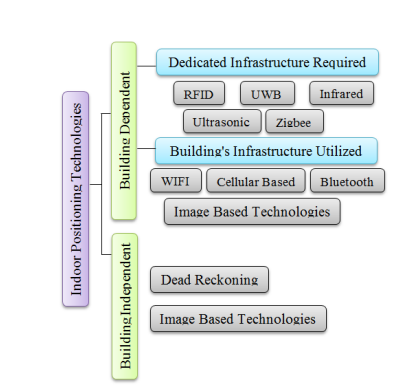
\includegraphics[scale=0.75]{classification_ips}
\caption{Classfication of indoor positioning technologies~\cite{ComparativeSurvey}}
\label{fig:ips_classification}
\end{figure}
\subsection{Wireless LAN}
\subsection{RFID}
\subsection{Bluetooth}
\subsection{Ultra-wideband}
\subsection{Infrared}
\subsection{Ultrasound}
\subsection{Zigbee}
\subsection{Cellular}
\subsection{Location Information for Positioning Systems}
There are four commonly used types of information for \acrshort{ips}\cite{Liu2007}.
\begin{enumerate}
\item Absolute location: the location as a point inside a reference grid, shared across all objects used in the space.
\item Physical location: location displayed as a point in a coordinate system (x, y, z), either 2D or 3D.
\item Symbolic location: translates a physical location into a more human centred location name, e.g. office 213 on the 1st floor.
\item Relative location: location is based on the relative distance or proximity to a beacon or base point, e.g. rescue helicopter flying over sea trying to locate any survivors.
\end{enumerate}
\section{Distance Measurement Techniques}
\begin{figure}[h!]
\centering
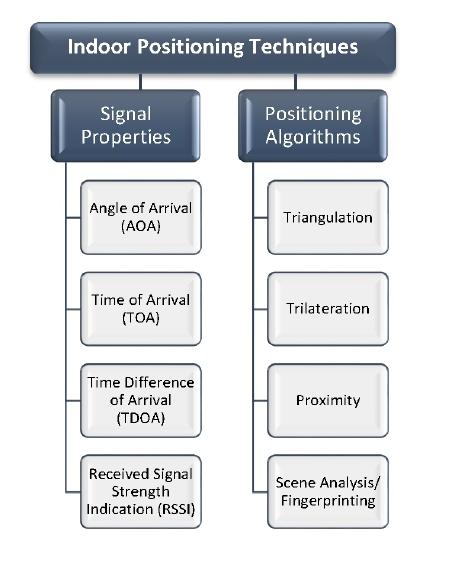
\includegraphics[scale=0.75]{classification_indoor_positioning_techniques}
\caption{Classification of indoor positioning techniques~\cite{Sakpere2017}}
\label{fig:ips_techniques}
\end{figure}
\subsection{Time of Arrival}
The \acrfull{toa} method is used to determine the distance between a \acrfull{tx} and \acrfull{rx}. In this method, the distance is calculated by the travelling time divided by the wave speed of the radio signal \cite{Loy2018}:
\begin{equation}
d = t * c
\end{equation}
Where d is the distance from \acrshort{tx} to \acrshort{rx} and c the constant speed of light (around $3.00 * 10^8 m/s$). This formula is based on research specifying the relationship between the propagation of a radio wave and its traversed range, which is a directly proportional relationship \cite{S2016}. Using the triangulation method for three available \acrlong{tx}s, the position of the \acrlong{rx} can be calculated. A synchronized clock is mandatory to provide accurate results, as the error rate is partially dependent on the speed of light, thus if there is an error of 1ms, the error in distance will be 300 meters. Hence the reason that \acrfull{gps} uses an atomic clock to ensure optimal accuracy \cite{Jindal}.
\begin{figure}[h!]
\centering
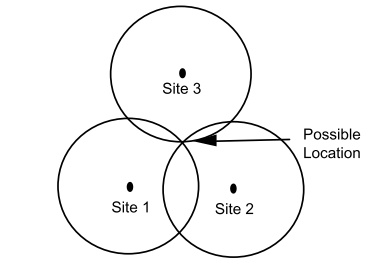
\includegraphics[scale=0.75]{toa}
\caption{Determining position in a two dimensional space by ~\acrlong{toa}~\cite{Jindal}}
\label{fig:toa}
\end{figure}
\subsection{Time Difference of Arrival}
\subsection{Angle of Arrival}
By using the \acrfull{aoa} method, the position of a device or \acrlong{mu} can be determined. This requires additional set up: directional antenna, thus \acrlong{tx}s. The intersection point of the lines indicating a direction signal resemble the possible location of the device, albeit without an exact error margin. The problem lies with the necessity of installing directional antenna arrays which contributes to higher cost than \acrlong{toa} and \acrlong{tdoa} \cite{Jindal}.
\begin{figure}[h!]
\centering
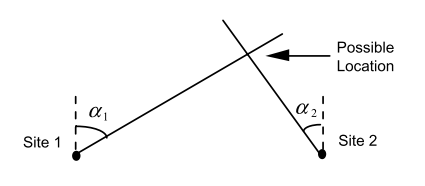
\includegraphics[scale=0.75]{aoa}
\caption{Determining position in a two dimensional space by ~\acrlong{aoa}~\cite{Jindal}}
\label{fig:aoa}
\end{figure}
\subsection{Received Signal Strength Indication}
\section{Indoor Positioning Techniques}
\subsection{Triangulation}
The angles of reference points are measured to calculate the position of the current position of the point, as visualized in \cite{fig:triang}. This method can only be used in combination with the distance method of \acrlong{aoa}.
\begin{figure}[h!]
\centering
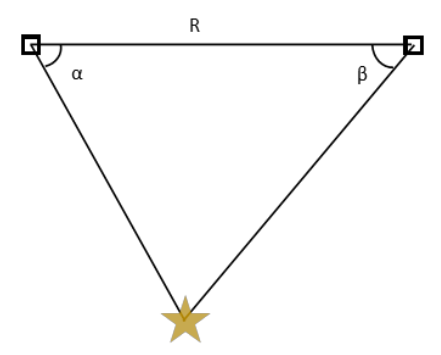
\includegraphics[scale=0.5]{triang}
\caption{Determining position using triangulation ~\cite{Loy2018}}
\label{fig:triang}
\end{figure}
\subsection{Trilateration}
\subsection{Scene Analysis/Fingerprinting}
\subsection{Proximity}
\section{Conclusion}
This thesis will cover the \acrshort{wlan} \acrlong{ips} technology and its implementation in a mobile application based on the provided project requirements.
